\section{The modular Bayesian framework}
\label{sec: model}

We develop a computational model to infer each learner’s internal processing states--specifically, their use of stimulus features during category learning--based solely on behavioral responses. Notably, the verbal reports collected during learning serve exclusively for model validation, providing \textbf{ground-truth benchmarks} to evaluate the model’s performance in predicting humans’ internal states.
As illustrated in Fig. \ref{fig:2}, we formulate the learner’s internal processing as trial-resolved Bayesian inference (Fig. \ref{fig:2}B) over a rich hypothesis space (Fig. \ref{fig:2}A), enabling comprehensive and coherent utilization of both stimulus properties and behavioral variability. We also implement three cognitively motivated components (perception, memory, and hypothesis generator) into the inference process to capture the bounded rationality of human learners (Fig. \ref{fig:2}C). This modular Bayesian framework generates eight model variants through module assembly (see Fig. \ref{fig:3}A), enabling systematic analysis of how individual cognitive factors--both independently and interactively--shape the learner's inference trajectory and observed behaviors, while enhancing explanatory power for the empirical phenomena.

% \vspace{1em}
\begin{figure}[htp!]
  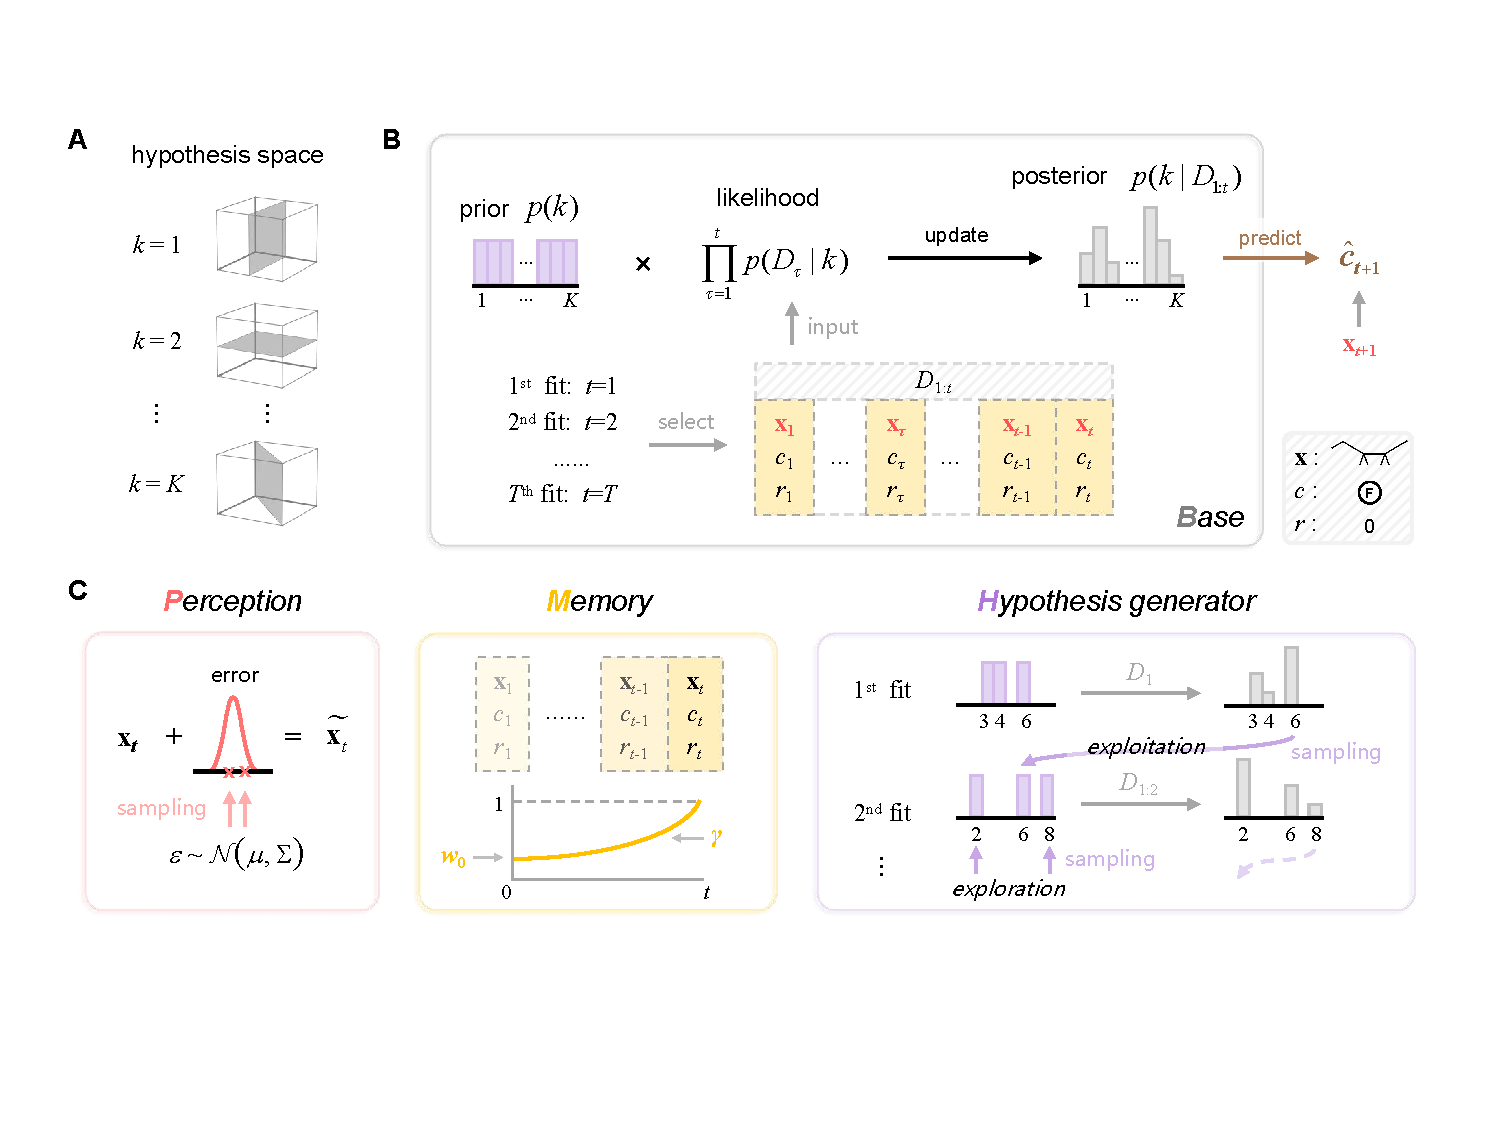
\includegraphics[width=1\textwidth, trim=1cm 2.7cm 1cm 2cm, clip]{figs/Figure2.pdf}
  \caption{Schematic of the Modular Bayesian framework. \textbf{(A)} Hypothesis space illustrated in a 3D feature space with two categories. Each hypothesis divides the space into two regions and assigns category probabilities to stimuli. \textbf{(B)} Bayesian inference engine in the rational backbone, serving as the baseline. Agents update their beliefs over hypotheses by integrating stimulus, choice, and feedback data. The resulting posterior is then used to predict the choice on the next trial. \textbf{(C)} Three bounded-rational modules augment the core inference in (B): a perception module adds Gaussian noise to stimulus input, a memory module down-weights past evidence via exponential decay, and a hypothesis generator adaptively samples a working hypothesis set through exploration–exploitation trade-offs.}
  \label{fig:2}
\end{figure}
% \vspace{1em}
\subsection{Rational backbone} \label{sec:3.1}

We posit that each learner entertains a library of geometric “partition” hypotheses that carve the four-dimensional feature space into regions associated with category labels, following classic concept-learning works showing that humans preferentially generate and test explicit rules (Bruner, Goodnow \& Austin 1956; Feldman 2000) rather than tuning infinitesimal weights. More importantly, Bayesian belief updating over this hypothesis space provides a normative engine that converts stimuli into graded category probabilities and refines those probabilities from trial to trial.

\textbf{Hypothesis space.} The \textit{hypothesis space} $\mathcal{H}$ is defined as a family of soft \textit{Voronoi} partitions mapping the \textit{feature space} $\mathbf X=[0,1]^D$ (here $D=4$) to the \textit{category probability space} $\Delta^{N-1}$ (with $N=2$ in Task 1 and $N=4$ in Tasks 2\&3). Each parametric partition $\theta \in \mathcal{H}$ is parameterized by a unique hard \textit{Voronoi} partition $k$, serving as the prototype, and a sharpness-coefficient $\beta>0$ that controls the softness of the decision boundary, thus $\theta=(k,\beta)$. For simplicity, we further restrict $k$ to a finite set $\mathcal{K}$ of geometrically regular partitions (see Fig. \ref{fig:2}A for an illustration in 3D space and Appendix B) and treat $\beta$ as an optimizable parameter, so that $|\mathcal{H}|=|\mathcal{K}|$. This keeps the hypothesis space expressive enough to approximate arbitrary decision surfaces, yet finite enough for efficient Bayesian updating on a trial-by-trial basis.
 
\textbf{Bayesian update.} Agents are initialized with a uniform prior over the discrete hypothesis prototypes, $p(k) = 1/|\mathcal{K}|$, and a uniform prior over the sharpness parameter, $\beta \in [\beta_{\min}, \beta_{\max}]$, which is used exclusively for optimization. By Bayes’ rule, the posterior over hypotheses $\theta$ after observing trial $t$ is updated as $p(\theta\mid\mathbf x_t,c_t,r_t)\;\propto\;p(\mathbf x_t,c_t,r_t\mid\theta)\;p(\theta)$, where $p(\theta)$ denotes the current prior belief over hypothesis $\theta$ and $p(\mathbf x_t,c_t,r_t\mid\theta)$ is the likelihood of the observed stimulus, choice, and feedback on trial $t$. This likelihood can be factorized as: 
\begin{equation}
    p(\mathbf{x}_t, c_t, r_t\mid\theta) = p(r \mid\mathbf{x}_t, c_t, \theta)\;p(c_t \mid\mathbf{x}_t, \theta)\;p(\mathbf{x}_t \mid\theta). \tag{1}
\end{equation}
Here, $p(c_t\mid\mathbf x_t,\theta)$ denotes the probability that a learner holding hypothesis $\theta$ would produce the observed choice $c_t$ when presented with stimulus $\mathbf x_t$. This probability is computed via the distances between the stimulus and the category centers specified by the partition $k$. $p(r_t \mid c_t, \mathbf{x}_t, \theta)$ and $p(\mathbf{x}_t \mid \theta)$ are defined by our experimental setup and independent of $\theta$. See Appendix B for further details.

Aggregating evidence up to trial $t$ (included), denoted as $\mathcal D_{1:t}\;=\;\bigl\{(\mathbf x_\tau,c_\tau,r_\tau)\bigr\}_{\tau=1}^{t}$,the log-posterior over hypothesis $\theta$ can be computed as (see Fig. \ref{fig:2}B):
\begin{equation}
    \log p(\theta\mid D_{1:t})=
    \log p(\theta)
    \;+\;
    \max_{\beta}\left(\sum_{\tau=1}^{t}w_\tau
        \log p(D_\tau\mid\theta)\right)
    \;-\;\log Z_t,
    \tag{2}
    \label{eq2}
\end{equation}
where ${{Z}_{t}}=p({{D}_{1:t}})$ is a normalization constant. The likelihood is $w_\tau$-weighted to account for imperfect memory (see Section \ref{sec:3.2}): $w_\tau = 1$ corresponds to fully rational Bayesian updating with perfect memory, while $w_\tau \le 1$ mimics human forgetting by down-weighting past evidence.

\subsection{Bounded-rational adaptations} \label{sec:3.2}
Three auxiliary modules are included to reconcile optimal computations with realistic human constraints(see Fig. \ref{fig:2}C). Specifically, the Perception module (P-module) accounts for uncertainty in sensory coding; a Memory module (M-module) captures information decay over time; and a Hypothesis generator module (H-module) imposes inductive bias by restricting the generation of candidate hypotheses. 

\textbf{Perception.} We assume that the features perceived by participants are corrupted by an independent Gaussian noise channel,
\begin{equation}
\tilde{\mathbf{x}}_t = \mathbf{x}_t + \boldsymbol{\varepsilon}, \qquad \boldsymbol{\varepsilon} \sim \mathcal{N}(\boldsymbol{\mu}, \boldsymbol{\Sigma}),
\tag{3}
\end{equation}
where $\boldsymbol{\mu}$ and $\boldsymbol{\Sigma}$ denote the feature-wise perceptual bias and variability, respectively, for each individual. These parameters are estimated from the Perception Calibration task (see Section ~\ref{sec: experiment} and Appendix A).

\textbf{Memory.} To account for imperfect memory, we down-weight older evidence via an exponential decay function, rescaling the log-likelihood sum in Eq.~\eqref{eq2}:
\begin{equation}
    w_j = w_0+\gamma^{t-j},\qquad 0\le\gamma,w_0\le 1 .
    \tag{4}
\end{equation}
Here $w_j$ quantifies the contribution of trial $j$ ($1 \le j \le t$) to the current log-posterior update at trial $t$. The parameter $\gamma$ controls the decay rate, with smaller values indicating faster forgetting, while $w_0$ captures a baseline memory trace--analogous to a long-term store that resists decay \cite{lewandowsky2009no}. By fitting $(\gamma,w_0)$ separately for each participant, the model can express a spectrum of recency effects and capture systematic individual differences in memory fidelity.

\textbf{Hypothesis generator.} Given cognitive capacity limits, learners likely operate on a dynamically updated subset of hypotheses--rather than maintaining the full hypothesis space as assumed in the rational backbone--as suggested by explorative behavioral patterns in Section ~\ref{sec: experiment}. We implement this process based on pre-defined sampling strategies and dynamically adjusted hypothesis-set sizes. 

We define three strategies for hypothesis selection: \textit{posterior-based exploitation} ($S_1$), \textit{cue-driven associative recall} ($S_2$), and \textit{stochastic exploration} ($S_3$). At every trial $t$ the learner firstly decides the amount of hypotheses to draw from each strategy, $(m_1^{(t)}, m_2^{(t)}, m_3^{(t)})$, then generates the next working hypothesis set $\mathcal H_{t+1}=\bigcup_{i=1}^3S_i^{(t)}$ from
\begin{align}
   \begin{aligned}  
   S_1^{(t)} &\in\left\{(\text{Top-}m_1^{(t)})(q_t(k);\mathcal{H}_{t}),\quad \text{No-Rep}(\pi(q_t(k)); m_1^{(t)})\right\}\\
   S_2^{(t)} &\in\left\{(\text{Top-}m_2^{(t)})(s_t(k|\mathbf{x}_{t+1});\mathcal{H}_{t}\backslash{S_1^{(t)}}),\quad \text{No-Rep}(\pi(s_t(k|\mathbf{x}_{t+1})); m_2^{(t)})\right\}\\
   S_3^{(t)} &\sim\text{Uniform}\!\left(\mathcal K\setminus(S_1^{(t)}\cup S_2^{(t)}),\;m_3^{(t)}\right) 
   \end{aligned}
   \tag{5}
\end{align}
where $q_t(k)$ is the current posterior and $s_t(k)$ denotes the associative similarity between the next stimulus $\mathbf x_{t+1}$ and partition $k$ (see details in Appendix B).

Remarkably, due to constraints inherent in human behavioral experiments, learning is typically observed as a one-shot trajectory sampling process--it is infeasible to collect repeated data from the same condition. Following prior work~\cite{gershman2015computational}, we incorporate a repeated sampling mechanism into the perception module and hypothesis generator to mitigate the randomness introduced by single-sample trajectories.


\subsection{Model fitting and comparison} \label{sec:3.3}
\textbf{Model space.} The full model space comprises the rational backbone (serving as the baseline model) combined with one, two, or all three bounded-rational adaptations, yielding eight candidate models. Systematic ablations allow us to attribute predictive gains to specific cognitive constraints.

\textbf{Optimization algorithms.}
We illustrate the optimization procedure using the full model (PMH-model). For each participant, we conduct a grid search over memory parameters $(\gamma, w_0)$ to maximize the posterior likelihood of their observed behavior. The resulting best-fit parameters are then used to generate 1000 simulated behavioral trajectories, from which the one that best matches the participant’s behavioral profile is selected (see Appendix B for details). For other reduced model variants, the same procedure is applied, with the corresponding cognitive module(s) omitted during optimization.

\begin{algorithm}
\caption{$PH_0M_0$ Model}
\begin{algorithmic}[1]
\Statex \textbf{Input:} $\bigl\{(\mathbf x_t,c_t,r_t)\bigr\}_{t=1}^{T},\mathcal{H},\gamma,w_0$
\Statex \textbf{Output:} ${(\hat{c_t})_{t=1}^T}, \bigr\{p_{post}^{(T)}(k)\bigr\}_{t=1}^T$
\Statex \textbf{Initialize:} $p_{post}^{(0)}(k) = \frac{1}{\left |\mathcal{H} \right |}$
\For{$t\gets1$ to $T_{max}$}
    \State $\hat{x} \gets x + \boldsymbol\varepsilon$
    \State $p_{post}^{(t+1)}(k)\gets Bayesian(p_{post}^{(t)}(k),\mathcal{H},\gamma,w_0)$
    \State $\hat{(c)}_{t} \sim \mathbb{E}_{p_{\text{post}}^{(t+1)}(k)} \left( \text{choice}(c \mid h,\vec{x}) \right)$
    \State $\mathcal{H} \gets$ Generate $\mathcal{H_{\text{new}}}$
\EndFor
\end{algorithmic}
\end{algorithm}

\textbf{Predictive assessment.}
We fit models using only behavioral data, while verbal reports collected during learning were used solely for validation, providing ground-truth benchmarks of participants’ internal states. To evaluate model alignment with both external behavior and internal representations, we computed two metrics: the mean absolute difference in learning performance (measured via sliding-window accuracy), and the difference in the probability assigned to the true hypothesis--estimated from model posteriors and participants’ verbal reports, respectively. Lower values on both metrics indicate better model-human alignment (see Appendix B for additional model fit indices).

